\documentclass{beamer}
\mode<presentation>
\usepackage{amsmath,amssymb,mathtools}
\usepackage{textcomp}
\usepackage{gensymb}
\usepackage{adjustbox}
\usepackage{subcaption}
\usepackage{enumitem}
\usepackage{multicol}
\usepackage{listings}
\usepackage{url}
\usepackage{graphicx} % <-- needed for images
\def\UrlBreaks{\do\/\do-}

\usetheme{Boadilla}
\usecolortheme{lily}
\setbeamertemplate{footline}{
  \leavevmode%
  \hbox{%
  \begin{beamercolorbox}[wd=\paperwidth,ht=2ex,dp=1ex,right]{author in head/foot}%
    \insertframenumber{} / \inserttotalframenumber\hspace*{2ex}
  \end{beamercolorbox}}%
  \vskip0pt%
}
\setbeamertemplate{navigation symbols}{}

\lstset{
  frame=single,
  breaklines=true,
  columns=fullflexible,
  basicstyle=\ttfamily\tiny   % tiny font so code fits
}

\numberwithin{equation}{section}

% ---- your macros ----
\providecommand{\nCr}[2]{\,^{#1}C_{#2}}
\providecommand{\nPr}[2]{\,^{#1}P_{#2}}
\providecommand{\mbf}{\mathbf}
\providecommand{\pr}[1]{\ensuremath{\Pr\left(#1\right)}}
\providecommand{\qfunc}[1]{\ensuremath{Q\left(#1\right)}}
\providecommand{\sbrak}[1]{\ensuremath{{}\left[#1\right]}}
\providecommand{\lsbrak}[1]{\ensuremath{{}\left[#1\right.}}
\providecommand{\rsbrak}[1]{\ensuremath{\left.#1\right]}}
\providecommand{\brak}[1]{\ensuremath{\left(#1\right)}}
\providecommand{\lbrak}[1]{\ensuremath{\left(#1\right.}}
\providecommand{\rbrak}[1]{\ensuremath{\left.#1\right)}}
\providecommand{\cbrak}[1]{\ensuremath{\left\{#1\right\}}}
\providecommand{\lcbrak}[1]{\ensuremath{\left\{#1\right.}}
\providecommand{\rcbrak}[1]{\ensuremath{\left.#1\right\}}}
\theoremstyle{remark}
\newtheorem{rem}{Remark}
\newcommand{\sgn}{\mathop{\mathrm{sgn}}}
\providecommand{\abs}[1]{\left\vert#1\right\vert}
\providecommand{\res}[1]{\Res\displaylimits_{#1}}
\providecommand{\norm}[1]{\lVert#1\rVert}
\providecommand{\mtx}[1]{\mathbf{#1}}
\providecommand{\mean}[1]{E\left[ #1 \right]}
\providecommand{\fourier}{\overset{\mathcal{F}}{ \rightleftharpoons}}
\providecommand{\system}{\overset{\mathcal{H}}{ \longleftrightarrow}}
\providecommand{\dec}[2]{\ensuremath{\overset{#1}{\underset{#2}{\gtrless}}}}
\newcommand{\myvec}[1]{\ensuremath{\begin{pmatrix}#1\end{pmatrix}}}
\let\vec\mathbf

\title{Matgeo Presentation - Problem 12.180}
\author{ee25btech11063 - Vejith}

\begin{document}


\frame{\titlepage}
\begin{frame}{Question}
    The system of linear equations\\
\hspace*{3cm}4x+2y=7\\
\hspace*{3cm}2x+y=6  has 
\begin{multicols}{2}
\begin{enumerate}[label=\alph*)]
    \item a  unique solution
    \item no solution
    \item infinite number of solutions
    \item exactly two distinct solutions 
\end{enumerate}
\end{multicols}
\end{frame}

\begin{frame}{Solution}
    Given linear equations are
\begin{align}
    \brak{4\hspace{0.5cm} 2}\myvec{x\\y}=7\\
     \brak{2\hspace{0.5cm} 1}\myvec{x\\y}=6
\end{align}
Equations (0.1) and (0.2) can be written as
\begin{align}
    \begin{pmatrix}
        4 & 2\\
        2 & 1
    \end{pmatrix} \myvec{x\\y}=\myvec{7\\6}
\end{align}
Forming the augmented matrix
\begin{align}
     \left(\begin{array}{cc|c}
        4 & 2 & 7 \\
        2 & 1 & 6 
\end{array}\right) &\xleftrightarrow{R_2 \rightarrow R_2- \frac{1}{2} \times R_1}  \left(\begin{array}{cc|c}
        4 & 2 & 7 \\
        0 & 0 & \frac{5}{2} 
\end{array}\right)
\end{align}
	As in the augmented matrix the entries of second  row are 0 their linear combination should also give 0 but it is $\frac{5}{2}$ which is a contradiction\\
$\implies$ So,the given system of linear equations has no solution
\end{frame}

\begin{frame}{Plot}
    \begin{figure}
    \centering
    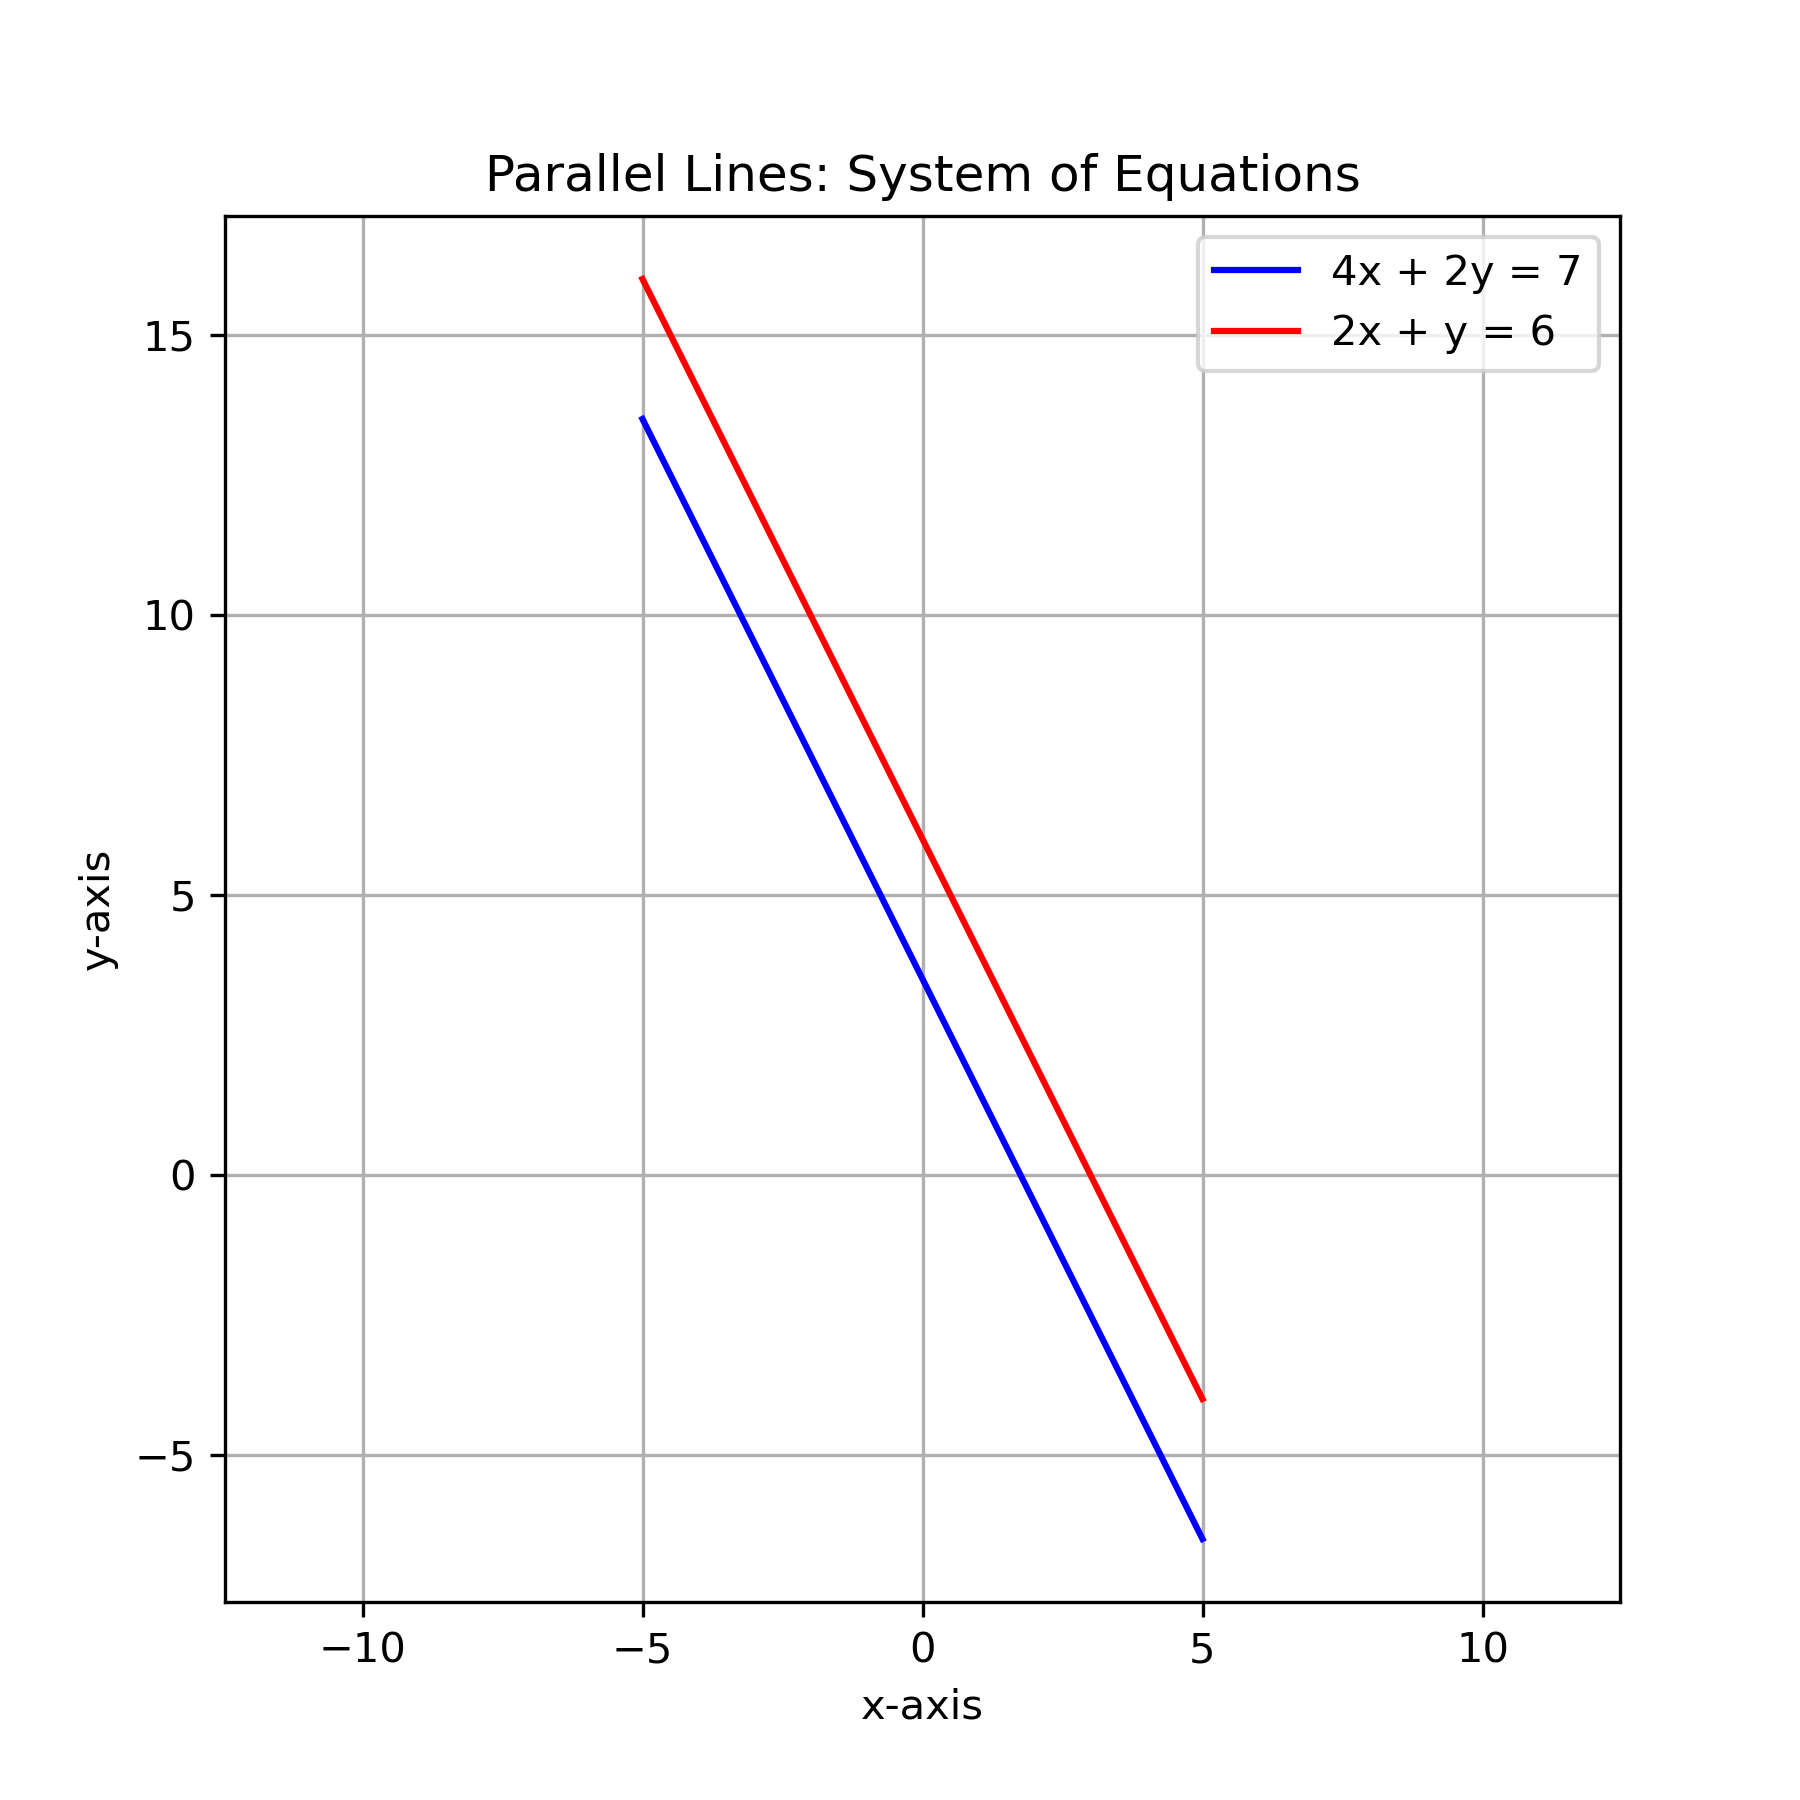
\includegraphics[width=0.7\columnwidth]{figs/01.png}
    \caption{}
    \label{fig:placeholder}
\end{figure}
\end{frame}

% --------- CODE APPENDIX ---------
\section*{Appendix: Code}

% C program
\begin{frame}[fragile]{C Code: Solution.c}
\begin{lstlisting}[language=C]
#include <stdio.h>

int main() {
    // Coefficients of equations:
    // Equation 1: 4x + 2y = 7
    // Equation 2: 2x +  y = 6
    int a1 = 4, b1 = 2, c1 = 7;
    int a2 = 2, b2 = 1, c2 = 6;

    // File pointer
    FILE *fp;
    fp = fopen("solution.dat", "w");
    if (fp == NULL) {
        printf("Error opening file!\n");
        return 1;
    }

    // Calculate determinants
    int det  = a1*b2 - a2*b1;   // determinant of coefficients
    int detx = c1*b2 - c2*b1;   // determinant replacing x-column
    int dety = a1*c2 - a2*c1;   // determinant replacing y-column

    if (det != 0) {
        // Unique solution exists
        double x = (double)detx / det;
        double y = (double)dety / det;
        fprintf(fp, "The system has a unique solution: x = %.2f, y = %.2f\n", x, y);
    }
    \end{lstlisting}
\end{frame}

\begin{frame}[fragile]{C Code: Solution.c}
\begin{lstlisting}[language=C]
    else {
        if (detx == 0 && dety == 0) {
            // Infinite solutions
            fprintf(fp, "The system has infinite number of solutions.\n");
        } else {
            // No solution
            fprintf(fp, "The system has no solution.\n");
        }
    }

    fclose(fp);
    return 0;
}

\end{lstlisting}
\end{frame}

% Python plotting
\begin{frame}[fragile]{Python: plot.py}
\begin{lstlisting}[language=Python]
import numpy as np
import matplotlib.pyplot as plt

# Define x range
x = np.linspace(-5, 5, 400)

# Line 1: 4x + 2y = 7 -> y = (7 - 4x) / 2
y1 = (7 - 4*x) / 2

# Line 2: 2x + y = 6 -> y = 6 - 2x
y2 = 6 - 2*x

# Plot the lines
plt.figure(figsize=(6,6))
plt.plot(x, y1, label="4x + 2y = 7", color="blue")
plt.plot(x, y2, label="2x + y = 6", color="red")

# Formatting
plt.xlabel("x-axis")
plt.ylabel("y-axis")
plt.title("Parallel Lines: System of Equations")
plt.legend()
plt.grid(True)
plt.axis("equal")

# Save the figure
plt.savefig("parallel_lines.png", dpi=300)

# Show the plot
plt.show()

\end{lstlisting}
\end{frame}
\end{document}
